\chapter{Resultados}
\label{chap:resultados}
\epigraph{There is no such thing as failure. There are only results.}{Tony Robbins}

En este cap\'{i}tulo se detallan los resultados obtenidos durante el experimento. Para las diferentes pruebas se utiliz\'{o} la c\'{a}mara \textit{Logitech} y la c\'{a}mara \textit{Minoru}. Se realiz\'{o} un total de 180 reconstrucciones utilizando la c\'{a}mara Logitech y un total de 120 reconstrucciones utilizando la c\'{a}mara Minoru. La diferencia en la cantidad se debe a que la c\'{a}mara Minoru s\'{o}lo soporta un m\'{a}ximo de 800x600 pixeles de resoluci\'{o}n por lo cual no pudo ser utilizada en reconstrucciones de 1024x768.

\section{Objetos del experimento}
Para el experimento se utilizaron dos objetos de forma, tama\~no y color diferentes. El primero es una r\'{e}plica de un castillo antiguo. En la figura ~\ref{fig:ResultsCastle} se muestran diferentes vistas de este objeto. Tiene un tama\~no aproximado de 17cm de alto, 9cm de ancho y 14cm de largo. Se encuentra construido de un tipo de resina y est\'{a} pintado con diferentes tonos de azules, verdes, rojos, amarillos y grises.


\begin{figure}[H]
\centering
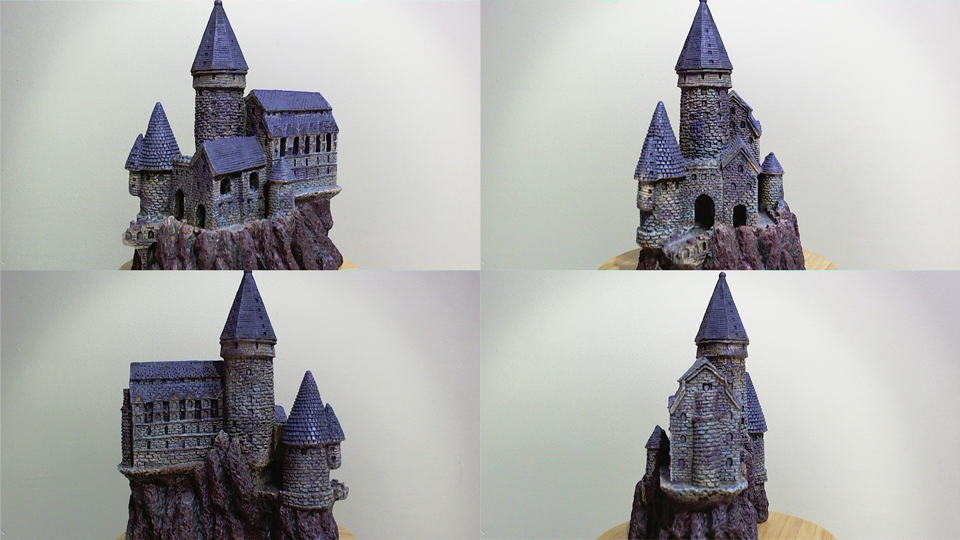
\includegraphics[width=1.0\textwidth]{images/castle.png}
\caption[R\'{e}plica miniatura de un castillo antiguo.]%
{R\'{e}plica miniatura de un castillo antiguo.}
\label{fig:ResultsCastle}
\end{figure}


El segundo objeto utilizado es una r\'{e}plica de unas columnas Griegas antiguas. En la figura ~\ref{fig:ResultsColumns} se muestran diferentes vistas de este objeto. Tiene un tama\~no aproximado de 17cm de alto, 21cm de ancho y 6cm de largo. Tambi\'{e}n se encuentra construido de un tipo de resina y est\'{a} pintado con diferentes tonos de caf\'{e} claro.


\begin{figure}[H]
\centering
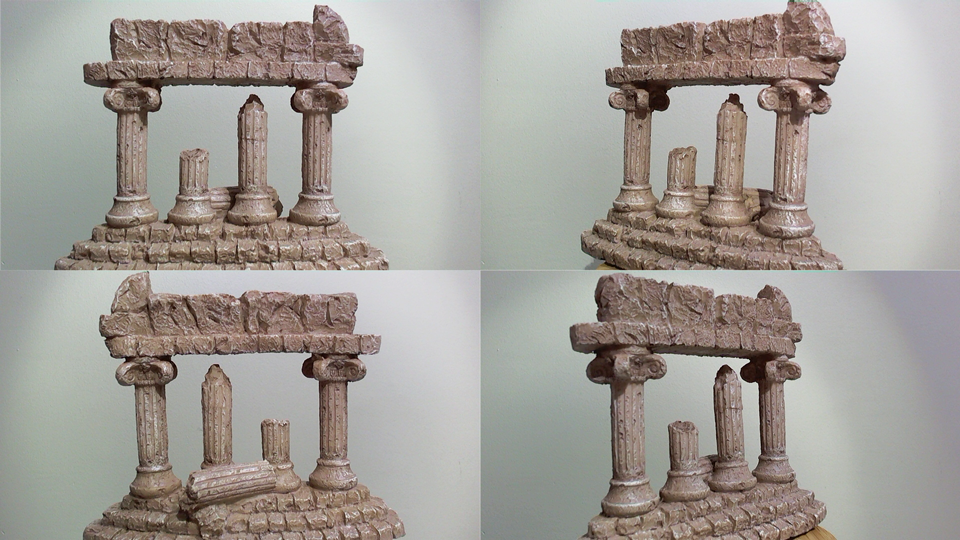
\includegraphics[width=1.0\textwidth]{images/greekcolumns.png}
\caption[R\'{e}plica miniatura de unas columnas Griegas]%
{R\'{e}plica miniatura de unas columnas Griegas.}
\label{fig:ResultsColumns}
\end{figure}

Se opt\'{o} por utilizar objetos cuya forma y color fueran considerablemente diferentes entre ellos con tal de observar el comportamiento del la t\'{e}cnica propuesta. A continuaci\'{o}n se muestran los resultados obtenidos a partir de un total de 300 reconstrucciones realizadas.


\section{Resoluci\'{o}n de im\'{a}genes vs. tiempo de reconstrucci\'{o}n}
Para la prueba se realiz\'{o} un total de 180 reconstrucciones (90 con el castillo y 90 con las columnas Griegas) utilizando la c\'{a}mara Logitech y un total de 120 reconstrucciones (60 con el castillo y 60 con las columnas Griegas) utilizando la c\'{a}mara Minoru. Se utilizaron tres diferentes resoluciones para la c\'{a}mara Logitech y dos para la c\'{a}mara Minoru. Por cada resoluci\'{o}n seleccionada se realizaron 30 reconstrucciones con ambas c\'{a}maras. Las resoluciones utilizadas fueron 640x480, 800x600 y 1024x768 para la c\'{a}mara Logitech mientras que para la c\'{a}mara Minoru se utiliz\'{o} \'{u}nicamente 640x480 y 800x600 debido a que no soporta 1024x768.

\begin{figure}[H]
\centering
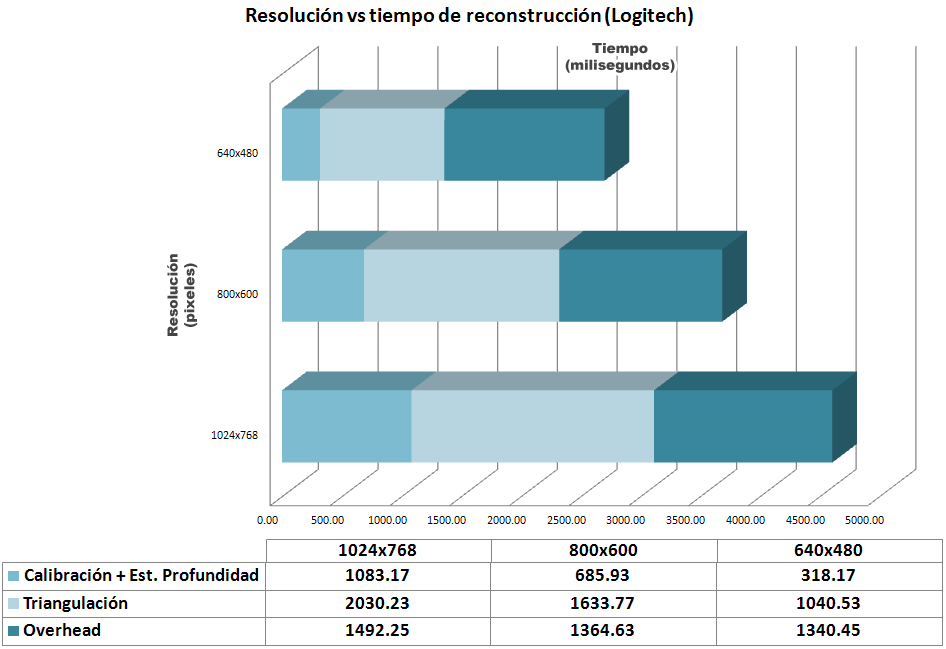
\includegraphics[width=1.0\textwidth]{images/chart-cl1.png}
\caption[Resoluci\'{o}n vs. tiempo de reconstrucci\'{o}n del castillo con la c\'{a}mara Logitech]%
{Resoluci\'{o}n vs. tiempo de reconstrucci\'{o}n del castillo con la c\'{a}mara Logitech. Los valores de tiempo est\'{a}n dados en milisegundos.}
\label{fig:ChartCL1}
\end{figure}


En la figura ~\ref{fig:ChartCL1} se muestran los resultados obtenidos a partir de 90 reconstrucciones realizadas al castillo desde todos los \'{a}ngulos posibles con la c\'{a}mara Logitech. La t\'{e}cnica se ejecut\'{o} 30 veces con capturas de 640x480 pixeles, 30 veces con capturas de 800x600 pixeles y finalmente, 30 veces con capturas de 1024x768 pixeles. La gr\'{a}fica muestra el promedio del tiempo total invertido (en milisegundos) en cada fase de la reconstrucci\'{o}n as\'{i} como el \textit{overhead} del experimento completo.


\begin{figure}[H]
\centering
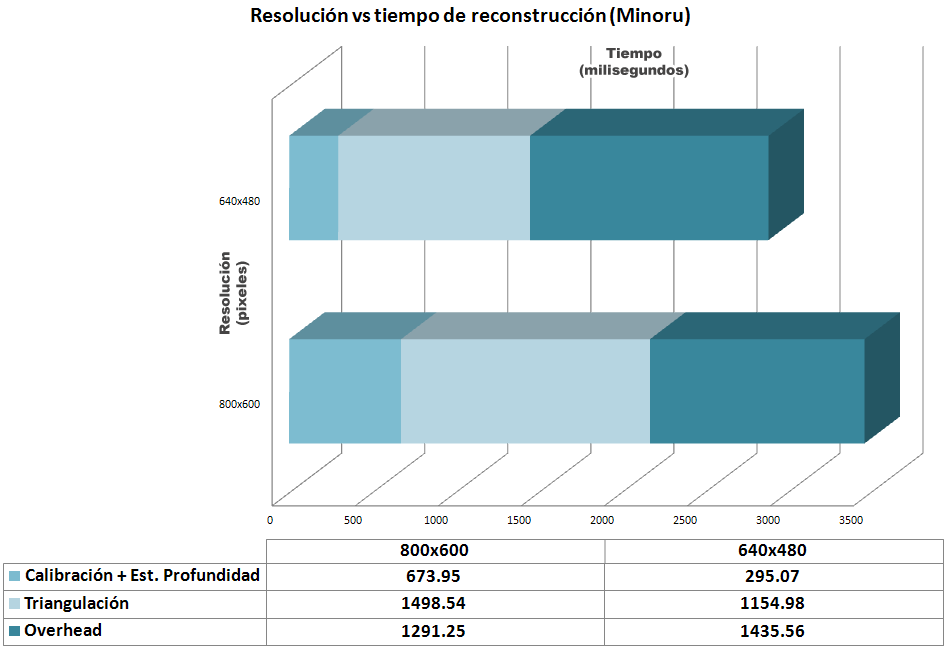
\includegraphics[width=1.0\textwidth]{images/chart-cm1.png}
\caption[Resoluci\'{o}n vs. tiempo de reconstrucci\'{o}n del castillo con la c\'{a}mara Minoru]%
{Resoluci\'{o}n vs. tiempo de reconstrucci\'{o}n del castillo con la c\'{a}mara Minoru. Los valores de tiempo est\'{a}n dados en milisegundos.}
\label{fig:ChartCM1}
\end{figure}


En la figura ~\ref{fig:ChartCM1} se muestran los resultados obtenidos a partir de 60 reconstrucciones realizadas al castillo desde todos los \'{a}ngulos posibles pero esta vez utilizando la c\'{a}mara Minoru. De igual forma, la t\'{e}cnica se ejecut\'{o} 30 veces con capturas de 640x480 pixeles y 30 veces con capturas de 800x600 pixeles. No fue posible ejecutarla con capturas de 1024x768 pixeles dado que la c\'{a}mara no soporta esa resoluci\'{o}n. La gr\'{a}fica muestra el promedio del tiempo total invertido (en milisegundos) en cada fase de la reconstrucci\'{o}n as\'{i} como el \textit{overhead} del experimento completo.


\begin{figure}[H]
\centering
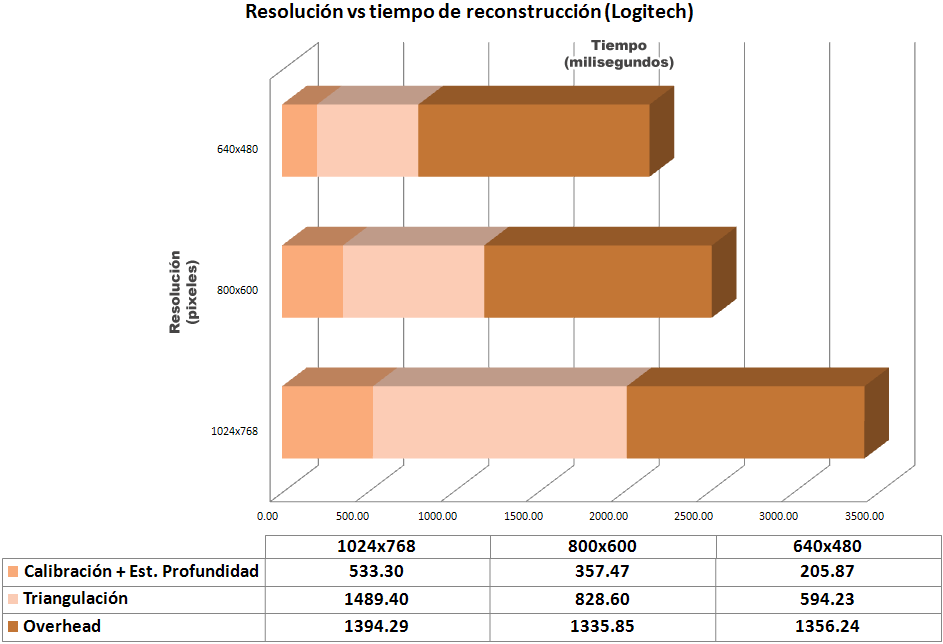
\includegraphics[width=1.0\textwidth]{images/chart-gl1.png}
\caption[Resoluci\'{o}n vs. tiempo de reconstrucci\'{o}n de las columnas Griegas con la c\'{a}mara Logitech]%
{Resoluci\'{o}n vs. tiempo de reconstrucci\'{o}n de las columnas Griegas con la c\'{a}mara Logitech. Los valores de tiempo est\'{a}n dados en milisegundos.}
\label{fig:ChartGL1}
\end{figure}


Seguidamente, se ejecut\'{o} la misma cantidad de reconstrucciones pero esta vez utilizando las columnas Griegas. En la figura ~\ref{fig:ChartGL1} se muestran los resultados obtenidos a partir de 90 reconstrucciones realizadas a las columnas desde todos los \'{a}ngulos posibles con la c\'{a}mara Logitech. Nuevamente, la t\'{e}cnica se ejecut\'{o} 30 veces con capturas de 640x480 pixeles, 30 veces con capturas de 800x600 pixeles y finalmente, 30 veces con capturas de 1024x768 pixeles.


\begin{figure}[H]
\centering
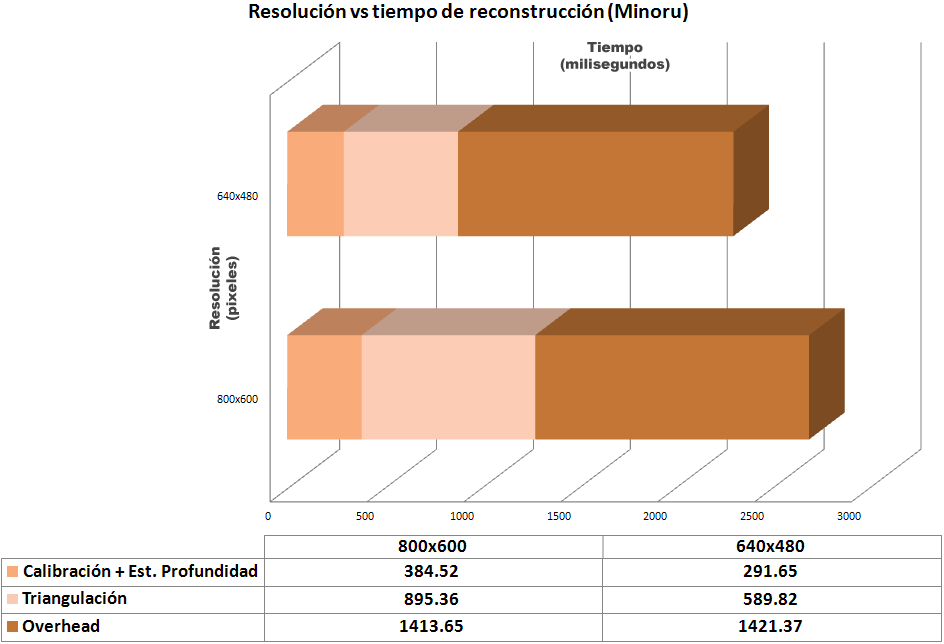
\includegraphics[width=1.0\textwidth]{images/chart-gm1.png}
\caption[Resoluci\'{o}n vs. tiempo de reconstrucci\'{o}n de las columnas Griegas con la c\'{a}mara Minoru]%
{Resoluci\'{o}n vs. tiempo de reconstrucci\'{o}n de las columnas Griegas con la c\'{a}mara Minoru. Los valores de tiempo est\'{a}n dados en milisegundos.}
\label{fig:ChartGM1}
\end{figure}


Finalmente, en la figura ~\ref{fig:ChartGM1} se muestran los resultados obtenidos a partir de las 60 reconstrucciones realizadas a las columnas desde todos los \'{a}ngulos posibles con la c\'{a}mara Minoru. De igual forma que con el castillo, la t\'{e}cnica se ejecut\'{o} 30 veces con capturas de 640x480 pixeles y 30 veces con capturas de 800x600 pixeles. No fue posible ejecutarla con capturas de 1024x768 pixeles debido a las limitaciones de la c\'{a}mara.


\section{Caracter\'{i}sticas f\'{i}sicas del objeto vs. tiempo de reconstrucci\'{o}n}
Para la prueba se utilizaron los mismos datos de las 300 reconstrucciones realizadas con ambas c\'{a}maras. Se utilizaron diferentes resoluciones para la c\'{a}mara Logitech y para la c\'{a}mara Minoru. Se contabiliz\'{o} el tiempo total de la reconstrucci\'{o}n y se promedi\'{o} la totalidad de los resultados para cada objeto.

\begin{figure}[H]
\centering
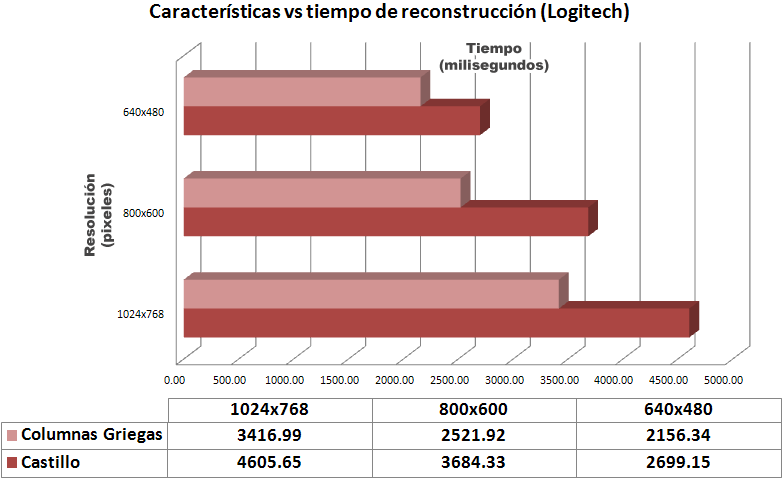
\includegraphics[width=1.0\textwidth]{images/featime1.png}
\caption[Caracter\'{i}sticas del objeto vs. tiempo de reconstrucci\'{o}n con la c\'{a}mara Logitech]%
{Caracter\'{i}sticas del objeto vs. tiempo de reconstrucci\'{o}n con la c\'{a}mara Logitech.}
\label{fig:FeatureVsTime1}
\end{figure}

En la figura ~\ref{fig:FeatureVsTime1} se muestran los resultados obtenidos con tres resoluciones 640x480, 800x600 y 1024x768 utilizando la c\'{a}mara Logitech con el castillo y las columnas Griegas.

\begin{figure}[H]
\centering
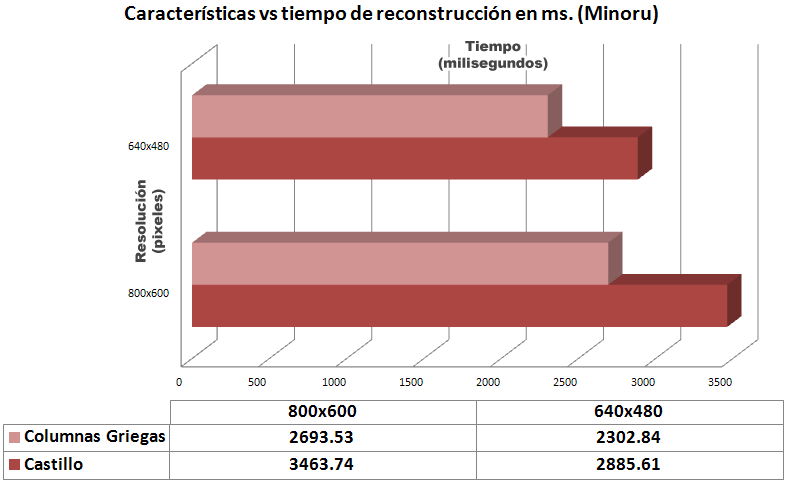
\includegraphics[width=1.0\textwidth]{images/featime2.png}
\caption[Caracter\'{i}sticas del objeto vs. tiempo de reconstrucci\'{o}n con la c\'{a}mara Minoru]%
{Caracter\'{i}sticas del objeto vs. tiempo de reconstrucci\'{o}n con la c\'{a}mara Minoru.}
\label{fig:FeatureVsTime2}
\end{figure}

Finalmente, en la figura ~\ref{fig:FeatureVsTime2} se muestran los resultados obtenidos para dos resoluciones 640x480 y 800x600 utilizando la c\'{a}mara Minoru nuevamente con el castillo y las columnas Griegas.


\section{Calibraci\'{o}n vs calidad de la reconstrucci\'{o}n}
Generalmente, cuando la calibraci\'{o}n falla los resultados obtenidos de la reconstrucci\'{o}n no se parecen en nada al objeto en cuesti\'{o}n. Fue necesario incorporar puntos de chequeo para determinar que los c\'{a}lculos obtenidos durante la fase de auto-calibraci\'{o}n (matrices \textit{P}) no sean totalmente err\'{o}neos. En la figura ~\ref{fig:WrongCalibration1} se muestra un ejemplo de una reconstrucci\'{o}n fallida del castillo por mala calibraci\'{o}n.

\begin{figure}[H]
\centering
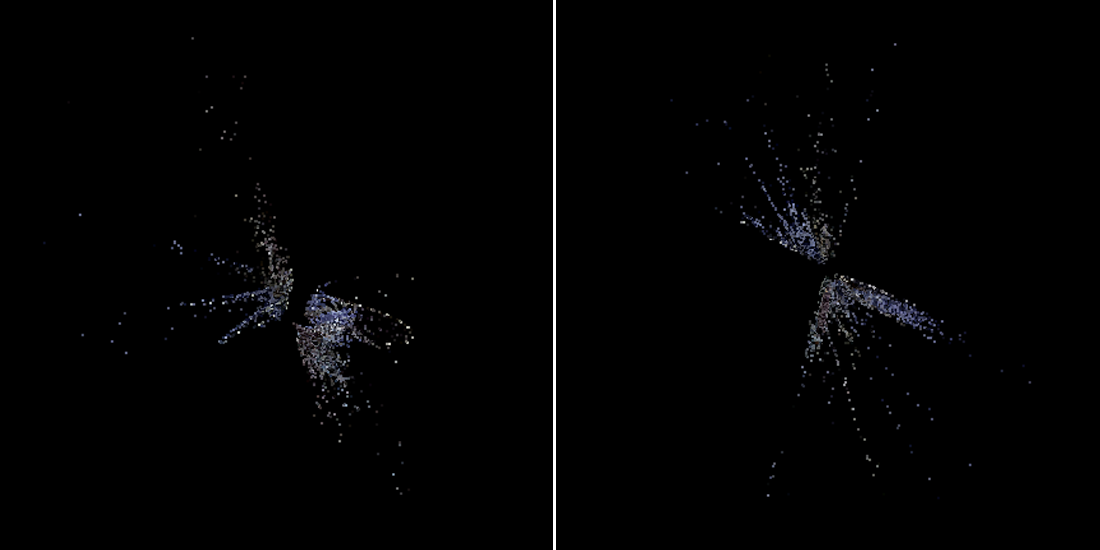
\includegraphics[width=1.0\textwidth]{images/wrongcal1.png}
\caption[Reconstrucci\'{o}n fallida del castillo]%
{Reconstrucci\'{o}n fallida del castillo. La imagen fue generada utilizando la t\'{e}cnica propuesta.}
\label{fig:WrongCalibration1}
\end{figure}

Otro ejemplo de reconstrucci\'{o}n fallida por mala calibraci\'{o}n se muestra en la figura ~\ref{fig:WrongCalibration2}. Esta vez, el objeto utilizado durante la reconstrucci\'{o}n fue el de las columnas Griegas.

\begin{figure}[H]
\centering
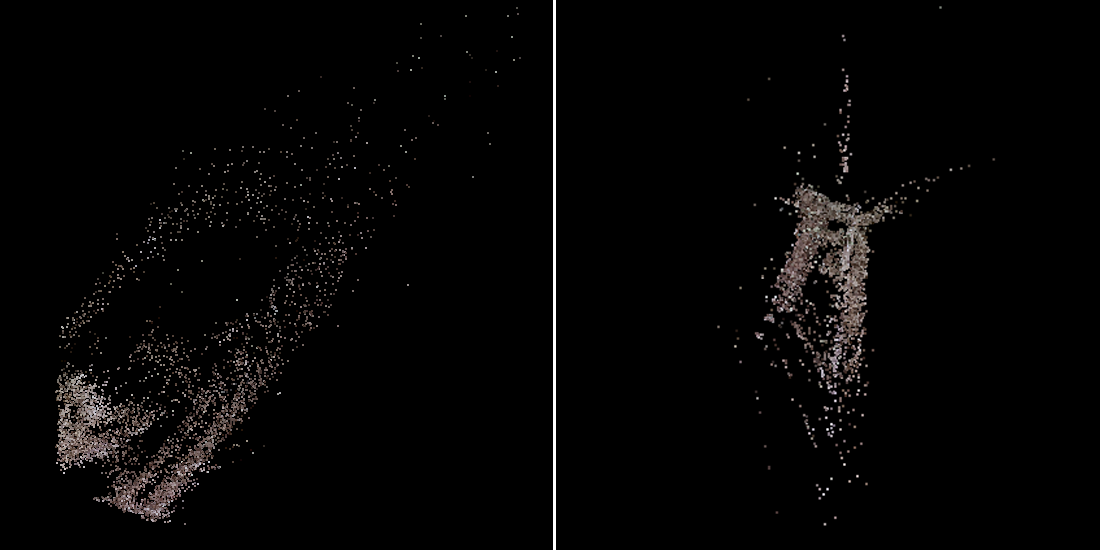
\includegraphics[width=1.0\textwidth]{images/wrongcal2.png}
\caption[Reconstrucci\'{o}n fallida de las columnas Griegas]%
{Reconstrucci\'{o}n fallida de las columnas Griegas. La imagen fue generada utilizando la t\'{e}cnica propuesta.}
\label{fig:WrongCalibration2}
\end{figure}

En la figura ~\ref{fig:CalibrationQuality} se muestra el porcentaje de fallos as\'{i} como la distribuci\'{o}n promedio en la calidad de las reconstrucciones obtenidas a partir de las 300 ejecuciones. Se le asign\'{o} un valor de 4 a una reconstrucci\'{o}n considerada como muy buena, 3 a una reconstrucci\'{o}n buena, 2 a una reconstrucci\'{o}n pobre y 1 a una reconstrucci\'{o}n mala (fallos).


\begin{figure}[H]
\centering
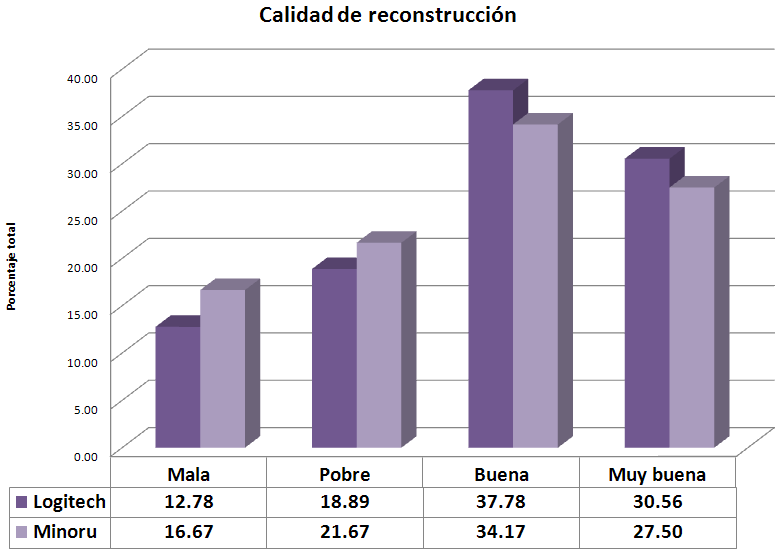
\includegraphics[width=1.0\textwidth]{images/calibquality1.png}
\caption[Calidad de la reconstrucci\'{o}n con ambas c\'{a}maras.]%
{Calidad de la reconstrucci\'{o}n con ambas c\'{a}maras.}
\label{fig:CalibrationQuality}
\end{figure}


Para efectos de comparaci\'{o}n se considera una reconstrucci\'{o}n mala cuando el resultado es totalmente incorrecto, como en el caso de las figuras ~\ref{fig:WrongCalibration1} y ~\ref{fig:WrongCalibration2}, una reconstrucci\'{o}n pobre cuando el resultado no es suficientemente denso y la distancia entre diferentes profundidades (por ej. las diferentes torres del castillo) no es cercana a la realidad del objeto, una reconstrucci\'{o}n buena cuando el resultado es denso y la distancia entre diferentes profundidades se asemeja m\'{a}s a la realidad del objeto. Finalmente, se considera una reconstrucci\'{o}n muy buena cuando los resultados son suficientemente densos y las m\'{e}tricas entre las diferentes profundidades son muy cercanas a la geometr\'{i}a real del objeto.


%A word of notice, many many times the reconstruction will fail because the Fundamental matrix came out wrong. The results will just look aweful, and nothing like a true reconstruction. To cope with this, you may want to insert a check that will make sure the two P matrices are not completely bogus (you could check for a reasonable rotation for example). If the P matrices, that are derived from the F matrix, are strange, then you can discard this F matrix and compute a new one.

